\documentclass[12pt,a4paper]{article}
\usepackage{fontawesome5}
\providecommand{\faPencilAlt}{\faIcon{pencil-alt}}
\usepackage{styles/couleurs}
\usepackage{styles/mise_en_page}
\usepackage{styles/boites}
\usepackage{styles/maths}
\usepackage{styles/figures}
\usepackage{enumitem}
\usepackage{array}
\usepackage{tabularx}
\usepackage{amsmath}
\usepackage{amssymb}
\usepackage{tikz}
\usepackage{xparse}
\usetikzlibrary{calc,patterns,arrows.meta}
\setlist[itemize]{leftmargin=1.4em,itemsep=0.15em,topsep=0.2em}
\setlist[enumerate]{leftmargin=*,itemsep=0.25em,topsep=0.25em}
\newcommand{\lignepointillee}{\noindent\dotfill\par\vspace{0.45em}}
\newcommand{\lignesreponse}[1]{%
\begin{tcolorbox}[enhanced,colback=white,colframe=NeutreC!40,boxrule=0.5pt,
arc=1.5mm,left=3mm,right=3mm,top=2mm,bottom=1mm,before skip=2pt,after skip=2pt]
\foreach \i in {1,...,#1}{\lignepointillee}
\end{tcolorbox}}
\newcommand{\titreseq}[1]{%
\begin{center}
{\sffamily\LARGE\bfseries\color{TitreC}Séquence 4 -- Calcul littéral}\\[0.2em]
{\sffamily\large\bfseries\color{SavoirC}#1}
\end{center}}
\begin{document}

\titreseq{Activité 6 -- Développer puis réduire}

On considère un rectangle de hauteur \(4\) cm et de longueur \(x+3\) cm.

\begin{center}
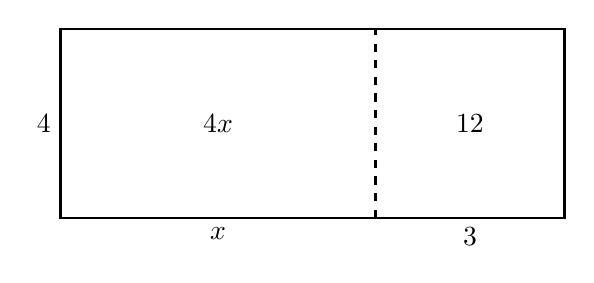
\begin{tikzpicture}[scale=0.8]
  \draw[line width=0.9pt] (0,0) rectangle (8,3);
  \draw[dashed,line width=0.8pt] (5,0)--(5,3);
  \node[below] at (2.5,0) {\(x\)};
  \node[below] at (6.5,0) {\(3\)};
  \node[left] at (0,1.5) {\(4\)};
  \node at (2.5,1.5) {\(4x\)};
  \node at (6.5,1.5) {\(12\)};
\end{tikzpicture}
\end{center}

\section*{Partie A -- Deux méthodes pour une même aire}

Écris l'aire :
\begin{enumerate}
  \item avec la longueur totale \(x+3\) ;
  \item en additionnant les aires des deux rectangles.
\end{enumerate}

\[
\dotfill
\]

Complète :

\[
4(x+3)=\ldots+\ldots
\]

\section*{Partie B -- Généraliser}

\begin{tcolorbox}[colback=SavoirC!5,colframe=SavoirC!60,boxrule=0.7pt,arc=2mm]
\[
k(a+b)=\dotfill
\]

\[
k(a-b)=\dotfill
\]

Développer, c'est transformer un \dotfill{} en une \dotfill
\end{tcolorbox}

\section*{Partie C -- Développer}

\[
A=5(x+2)
\qquad
B=3(2x+7)
\]

\[
C=-2(x+4)
\qquad
D=4(3x-5)
\]

\lignesreponse{6}

\section*{Partie D -- Développer puis réduire}

\[
E=3(x+4)+2x
\]

\[
F=5(2x-1)-3x
\]

\[
G=-2(x+3)+7x-4
\]

\[
H=4(2x-5)-3(x+1)
\]

\lignesreponse{9}

\section*{Partie E -- Vérifier}

Choisis une valeur de \(x\) et vérifie que \(G\) et sa forme réduite
ont la même valeur.

\lignesreponse{4}

\end{document}
